\documentclass[11pt]{article}
\usepackage[margin=.85in]{geometry}
\usepackage{amsmath,amssymb,booktabs,microtype,graphicx}
\usepackage{placeins}
\usepackage[hidelinks]{hyperref}
\usepackage{tikz}
\usetikzlibrary{arrows.meta,calc,positioning}

\title{\textbf{Natural-Sparsity Acceleration for Ternary LLMs}\\When Does a Compressed, Zero-Aware Matrix--Vector Engine Beat Five-Trit Packing?}
\author{Jacob Zymet\\Independent Researcher}
\date{September 2026\\[2pt]\small\textit{Preprint}}

\begin{document}
\maketitle

\begin{abstract}
Ternary large language models encode quantized weight symbols in $\{-1,0,+1\}$, reducing storage and replacing general per-weight multiplication with sign selection and zeroing. I test whether the natural, unstructured zeros in trained ternary models justify a presence-bitmap plus compact-sign representation and matching matrix--vector multiply (GEMV) datapath, without retraining or structured sparsity. I compare matched bitmap/sign and five-trit engines using RTL, timing-aware synthesis, static timing, and gate-level switching-energy analysis in Nangate45, including weight-feeding logic. The bitmap/sign engines reach 9--14\% shorter minimum clock periods. The byte-stream design is 11--31\% larger; the five-bit-presence design with its dedicated streaming loader is 23--36\% larger at the three power-study clocks. Both streamed designs use more compute energy because the five-trit decoder already suppresses zero weights before the shared adder tree. The bitmap representation becomes smaller than continuous five-trit packing above 40\% zeros, so any consistent energy gain comes from reduced memory traffic. Across 13 public checkpoints, nine quantization-aware or fine-tuned models contain 29--42\% zeros and save at most 1.3\% in the modeled projection path. Higher-zero CAT-Q Qwen3 checkpoints save 3.7--6.8\% for LPDDR4-streamed ternary-symbol weights, falling to about 1.9--2.1\% after scale and output-head reads are included. Natural ternary sparsity is therefore useful mainly when zero density is high and weight reads are expensive.
\end{abstract}

\section{Introduction}

Ternary transformer models encode many learned weights with quantized symbols
\begin{equation}
q \in \{-1,0,+1\},
\end{equation}
with scale factors handled separately. Multiplying by the ternary symbol therefore means selecting $x$, $-x$, or zero rather than performing a general per-weight multiplication. BitNet established that this representation can scale to language models while remaining competitive with higher-precision baselines \cite{wang2025bitnet}. Software runtimes such as bitnet.cpp further show that specialized ternary kernels can provide substantial inference benefits on conventional processors \cite{wang2025bitnetcpp}. For batch-1 decoding, each weight matrix is multiplied by a single activation vector. In the streaming model used here, every modeled weight is read once per generated token, so weight traffic is a central cost. KV-cache traffic, activation traffic, and other non-weight memory traffic are outside the model.

Specialized ternary hardware already exists. Slim-Llama demonstrated a fabricated binary/ternary LLM processor at ISSCC 2025 \cite{kim2025slimllama}, and later work explored lookup-table (LUT) accelerators \cite{huang2025tenet,geens2026lut}, FPGA systems \cite{qiao2025tellme}, compute-in-ROM \cite{zhang2026bitrom}, sparse ternary matrix--matrix multiplication (GEMM) \cite{pittet2026ssr,zhu2026sparsegemm}, packed post-training-quantized weights \cite{jung2026tace}, and a 16 nm ternary/mixed-precision silicon prototype in VitaLLM \cite{lin2026vitallm}. I instead test whether the \emph{natural} zeros already present in pretrained ternary LLMs justify changing the physical weight representation and datapath.

Georganas et al. measured 29 ternary LLM checkpoints (published sets of trained weights) and found that roughly $29.7\%$ to $51.5\%$ of their weights were zero \cite{georganas2026bitcos}. Their BITCOS representation stores one presence bit per weight and one sign bit per nonzero weight. If the fraction of zero weights is $z$, the storage required is
\begin{equation}
B_{\mathrm{bitmap}}(z)=2-z
\end{equation}
bits per weight. It becomes smaller than five-trit packing when five-trit packing restarts every 128 weights (1.625 bits per weight) at
\begin{equation}
z>0.375.
\end{equation}
For continuous five-trit packing at exactly 1.6 bits per weight, used as the stronger baseline in the main experiments below, the bitmap representation becomes smaller when $z>0.4$.

Storage savings alone are not enough. Bitmap/sign encoding requires extra logic to find each nonzero weight's sign in the compacted sign stream, and irregular zero locations can increase routing overhead and leave hardware underused. BITCOS also shows on CPUs that a smaller representation can perform worse when decoding becomes the bottleneck instead of memory bandwidth \cite{georganas2026bitcos}. I therefore compare matched bitmap/sign and five-trit hardware, including the logic needed to supply both designs with weights from memory. The study contributes:
\begin{itemize}
\item RTL engines that directly use the presence-bitmap and compact-sign format, with presence bits gating the activations, using two ways of supplying weights from memory. These are compared with a five-trit engine of equal throughput under identical synthesis, static timing, and gate-level power analysis in Nangate45, including the hardware that feeds each engine from memory.
\item A timing-aware comparison of the area and clock-speed trade-off, showing that area-only synthesis would have reversed the area conclusion.
\item A gate-level energy breakdown showing why the presence mask removes no additional adder-tree arithmetic: the five-trit decoder already turns zero weights into zero lane contributions before the same tree.
\item A break-even relationship between the fraction of zero weights and memory energy per bit.
\item Exhaustive ternary-projection zero statistics for 13 public checkpoints and a model-wide estimate of projection-engine plus ternary-symbol weight-read energy per decoded token.
\end{itemize}
The result is mostly negative. The bitmap/sign engine is faster, but it is larger and does not show a consistent compute-energy advantage, so its main energy benefit comes from reading fewer bits from memory. The bitmap/sign representation becomes smaller above 40\% zeros, and the benefit grows as weight reads become more expensive. The quantization-aware or fine-tuned models tested here provide little or no gain; the higher-zero CAT-Q Qwen3 models reach a few percent.

\section{Related work}

\subsection{Ternary accelerator ASICs}

Slim-Llama uses binary/ternary quantization and sparsity-aware lookup-table execution in a fabricated LLM processor \cite{kim2025slimllama}. VitaLLM combines a multiplier-free ternary core with mixed-precision attention hardware in a 16 nm silicon prototype \cite{lin2026vitallm}.

\subsection{LUT and packed ternary execution}

TENET proposes a sparse-aware LUT-centric architecture with ternary weight decompression and activation sparsity \cite{huang2025tenet}. Geens et al. systematically explore the LUT accelerator design space and show that the best organization strongly depends on activation precision \cite{geens2026lut}. T-ACE co-packs ternary weights with scale metadata and overlaps five-trit decoding with GEMM execution \cite{jung2026tace}. Packing five ternary symbols per byte and decoding them in hardware are established: TENET includes ternary weight decompression \cite{huang2025tenet}, TerEffic stores five ternary weights per byte and decodes them to five two-bit weights on FPGA \cite{yin2025tereffic}, and T-ACE uses a two-stage five-trit unpacker \cite{jung2026tace}. Platinum likewise uses 1.6-bit ternary packing in its LUT-based accelerator \cite{shan2026platinum}. Platinum also reports that DRAM and weight-buffer accesses account for 53.5\% and 31.6\% of its power \cite{shan2026platinum}. Five-trit packing is therefore a strong baseline.

\subsection{Sparse ternary computation}

SSR and addition-based sparse GEMM explicitly exploit zero ternary weights \cite{pittet2026ssr,zhu2026sparsegemm}. Sparse-BitNet and Sherry instead create hardware-friendly structured sparsity during training \cite{zhang2026sparsebitnet,huang2026sherry}. SparseBits combines learned sparsification, block scheduling, bitmap encoding, and an accelerator for BitNet's ternary layers \cite{song2026sparsebits}. SATLLM from the same group likewise proposes a sparsity-aware accelerator for ternary-weight LLMs \cite{liu2026satllm}. Slim-Llama instead generates 62.3\% sparsity for its ternary Llama benchmark by reusing outputs of similar weight vectors \cite{kim2025slimllamahc}.

I do not introduce sparsity, retrain the model, or change its weights. The input is an already-trained ternary tensor with arbitrary natural zero locations. I test whether that exact tensor can be executed more efficiently from its compressed representation.

\subsection{Natural ternary sparsity}

BITCOS provides the closest prior work on this representation \cite{georganas2026bitcos}. It is lossless and requires no retraining, and it is evaluated only in CPU and GPU software. The highest zero fraction in its survey, 51.5\%, comes from a CAT-Q model. CAT-Q converts pretrained full-precision LLMs to ternary weights after training, with a learned threshold and one scale per group of 128 weights \cite{wang2026catq}, and its checkpoints are public. TOM exploits ternary zero weights in hardware by synthesizing a read-only weight memory as logic rather than streaming compressed weights \cite{guan2026tom}. TENET gates computation when an entire weight group is zero \cite{huang2025tenet}. The present study instead asks whether arbitrary element-level natural zeros can be exploited directly. BITCOS reports a BitNet b1.58 zero density of $z=0.4219$ \cite{georganas2026bitcos}, which implies
\begin{equation}
B_{\mathrm{bitmap}}=1.5781
\end{equation}
symbol bits per weight, compared with $1.625$ for five-trit packing.

That difference is only about $2.9\%$. Whether it offsets the bitmap engine's additional decoding and feeding energy depends on the cost of each weight read. Compression alone can yield a net energy saving when reads are sufficiently expensive, as the results below quantify.

\section{Architectures}
\label{sec:arch}

All engines accept one group of five weight positions and five 8-bit signed activations per cycle, sum the five signed contributions in the same signed adder tree, and accumulate a 24-bit row result, so they have the same steady-state throughput of five positions per accepted cycle. They were verified against an exact integer reference.


Figure~\ref{fig:architecture-overview} summarizes the matched datapaths. Both produce five signed-or-zero activation values and sum them with the same structure; the difference is how each weight representation supplies those values.

\begin{figure}[t]
\centering
\resizebox{\linewidth}{!}{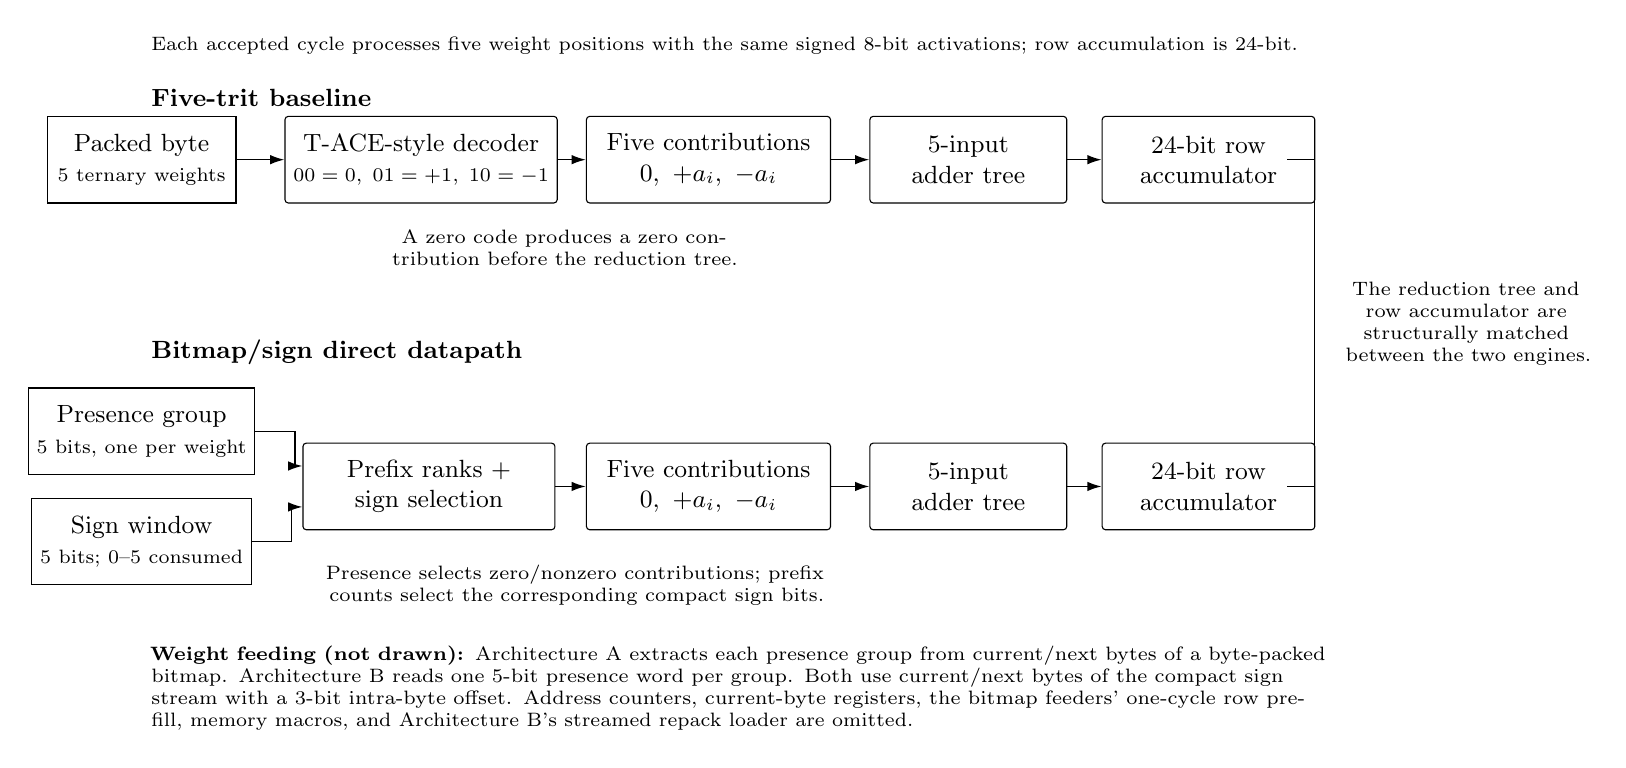
\begin{tikzpicture}[
  font=\small,
  box/.style={draw, rounded corners=1.2pt, minimum height=11mm, align=center, inner sep=3pt},
  src/.style={draw, minimum height=11mm, align=center, inner sep=3pt},
  arr/.style={-{Latex[length=1.8mm,width=1.2mm]}, line width=0.55pt},
  note/.style={font=\scriptsize, align=center},
  head/.style={font=\bfseries\small, anchor=west}
]

% Global scope note
\node[note, anchor=west] at (0,1.45)
  {Each accepted cycle processes five weight positions with the same signed 8-bit activations; row accumulation is 24-bit.};

% Five-trit baseline
\node[head] at (0,0.78) {Five-trit baseline};
\node[src, minimum width=24mm] (ftin) at (0,0) {Packed byte\\\scriptsize 5 ternary weights};
\node[box, minimum width=31mm] (ftdec) at (3.55,0) {T-ACE-style decoder\\\scriptsize $00=0,\;01=+1,\;10=-1$};
\node[box, minimum width=31mm] (ftcontrib) at (7.20,0) {Five contributions\\$0,\ +a_i,\ -a_i$};
\node[box, minimum width=25mm] (fttree) at (10.50,0) {5-input\\adder tree};
\node[box, minimum width=27mm] (ftacc) at (13.55,0) {24-bit row\\accumulator};

\draw[arr] (ftin) -- (ftdec);
\draw[arr] (ftdec) -- (ftcontrib);
\draw[arr] (ftcontrib) -- (fttree);
\draw[arr] (fttree) -- (ftacc);

\node[note, anchor=north, text width=60mm] at (5.35,-0.77)
  {A zero code produces a zero contribution before the reduction tree.};

% Bitmap/sign direct datapath
\node[head] at (0,-2.45) {Bitmap/sign direct datapath};
\node[src, minimum width=25mm] (pres) at (0,-3.45) {Presence group\\\scriptsize 5 bits, one per weight};
\node[src, minimum width=25mm] (sign) at (0,-4.85) {Sign window\\\scriptsize 5 bits; 0--5 consumed};
\node[box, minimum width=32mm] (align) at (3.65,-4.15) {Prefix ranks +\\sign selection};
\node[box, minimum width=31mm] (bscontrib) at (7.20,-4.15) {Five contributions\\$0,\ +a_i,\ -a_i$};
\node[box, minimum width=25mm] (bstree) at (10.50,-4.15) {5-input\\adder tree};
\node[box, minimum width=27mm] (bsacc) at (13.55,-4.15) {24-bit row\\accumulator};

\draw[arr] (pres.east) -- ++(5mm,0) |- ($(align.west)+(0,2.6mm)$);
\draw[arr] (sign.east) -- ++(5mm,0) |- ($(align.west)+(0,-2.6mm)$);
\draw[arr] (align) -- (bscontrib);
\draw[arr] (bscontrib) -- (bstree);
\draw[arr] (bstree) -- (bsacc);

\node[note, anchor=north, text width=73mm] at (5.50,-5.02)
  {Presence selects zero/nonzero contributions; prefix counts select the corresponding compact sign bits.};

% Matched arithmetic note
\node[note, anchor=west, text width=31mm] at (15.15,-2.08)
  {The reduction tree and row accumulator are structurally matched between the two engines.};
\draw[line width=0.45pt] (14.55,0.00) -- (14.90,0.00) -- (14.90,-4.15) -- (14.55,-4.15);

% Weight-feeding scope
\node[note, anchor=north west, text width=150mm, align=left] at (0,-6.05)
  {\textbf{Weight feeding (not drawn):} Architecture A extracts each presence group from current/next bytes of a byte-packed bitmap. Architecture B reads one 5-bit presence word per group. Both use current/next bytes of the compact sign stream with a 3-bit intra-byte offset. Address counters, current-byte registers, the bitmap feeders' one-cycle row prefill, memory macros, and Architecture B's streamed repack loader are omitted.};

\end{tikzpicture}
}
\caption{Conceptual comparison of the matched five-trit and direct bitmap/sign datapaths. Both form five signed-or-zero activation contributions and reduce them with the same five-input adder-tree structure; the difference is the front end that reconstructs those contributions from the stored weight representation. Feeding details for Architectures A and B are summarized below the datapaths.}
\label{fig:architecture-overview}
\end{figure}

\subsection{Five-trit baseline}

Five ternary weights are packed into one byte ($3^5=243\le256$), 1.6 bits per weight. A replicated T-ACE-style decoder \cite{jung2026tace} turns the byte into five two-bit codes (add, subtract, zero), and a zero code blocks its activation from the adder tree. When fed from memory, the engine needs only a byte address counter: the memory output register holds the current group's byte and drives the decoder directly.

\subsection{Fused bitmap/sign engine}

The weights are stored as a presence bitmap (one bit per weight) and a compact sign stream (one bit per nonzero weight). Each cycle takes five presence bits and between zero and five sign bits. The presence bits gate the activations directly; for each present position the prefix count of presence bits below it selects its sign from a window of the sign stream. The datapath never reconstructs a two-bit weight vector. The inner operation is
\begin{equation}
y \mathrel{+}= 
\begin{cases}
+x_i, & p_i=1,\ s_{r(i)}=+,\\
-x_i, & p_i=1,\ s_{r(i)}=-,\\
0, & p_i=0,
\end{cases}
\end{equation}
where $p_i$ is the presence bit and $r(i)$ is the rank of position $i$ among nonzero entries in the current group, offset by the sign-stream position at the start of the group.

Two decoded variants reconstruct a two-bit weight vector before the adder tree. The ``presence extracted'' variant receives five already-aligned presence bits and excludes presence-byte alignment, so it has a different input boundary from the direct engine. The ``full-front decoded'' variant includes the same presence-byte alignment as the direct engine and provides the matched comparison of decoded and fused compute. Both decoded variants were evaluated for area and timing only.

\subsection{Feeding the bitmap/sign engine}

Both streams live in memories with one synchronous read port and a one-cycle read delay; the memories themselves are outside the synthesized designs, whose weight-feeding logic is included.

\textbf{Architecture A (two byte streams).} Each stream is byte-wide. Per stream the engine keeps a byte address counter and a current-byte register and reads a 16-bit window of current and next byte; the presence stream advances five bits per group and the sign stream a data-dependent zero to five bits. Rows start at arbitrary bit addresses, a start cycle followed by one idle prefill cycle is needed per row, and the design sustains one group per cycle with no stalls for any weight pattern.

\textbf{Architecture B (five-bit presence memory).} The presence bits are stored in a memory with five-bit words, read once per group exactly like five-trit's bytes, so the presence side needs only an address counter; the sign stream is fed as in Architecture A. Each row's presence bits are zero-padded to a multiple of five before byte packing; the sign stream remains compact and continuous. A loader repacks this byte-packed bitmap into the memory (five input bytes become eight five-bit words). If the compressed weights remain resident in on-chip banks (five-bit presence words and byte-wide signs), the loader is idle during inference (``B resident''). If byte-packed weights are streamed in during inference, the loader operates at the stream rate and its area and energy are charged to the engine (``B streamed'').

\section{Methodology}
\label{sec:method}

\subsection{Real model traces}

I analyzed every projection weight in every layer of 13 public ternary checkpoints, using pinned Hugging Face revisions with file hashes checked against the Hub. Nine were made by quantization-aware training or fine-tuning, in which the model learns with ternary weights: BitNet b1.58 2B4T \cite{ma2025bitnet2b4t}, the \texttt{1bitLLM} reproduction \texttt{bitnet\_b1\_58-large} \cite{ma2024era}, TriLM 1.1B \cite{kaushal2024spectra}, Falcon-E 1B and 3B \cite{falcone2025}, the 1.58-bit Falcon3 1B, 3B and 7B \cite{falcon3blog2024}, and \texttt{HF1BitLLM/Llama3-8B-1.58-100B-tokens} \cite{mekkouri2024finetuning}. Four were ternarized after training by CAT-Q \cite{wang2026catq}: Qwen3 1.7B, 4B and 8B and Llama2-7B. Seven of the nine quantization-aware or fine-tuned checkpoints and all four CAT-Q checkpoints store packed ternary codes, which are decoded exactly (CAT-Q's group-128 format stores one 16-bit scale and 128 two-bit codes per group; no group has a zero or negative scale). TriLM stores weights already ternarized as $\{0,\pm s\}$. Only \texttt{bitnet\_b1\_58-large} stores full-precision latent weights, which were quantized with the BitNet absmean rule (divide by the mean absolute weight of the tensor and round to $-1$, $0$ or $+1$); on two BitNet 2B4T layers, applying the same rule to the published full-precision weights reproduces the packed ternary weights except for 0.72\% of weights, all within $\pm 1/256$ of the rounding threshold and with no sign disagreements. Two independent checks agree with published figures: the CAT-Q Qwen3-1.7B zero fraction matches the 51.48\% reported by BITCOS \cite{georganas2026bitcos}, and the CAT-Q Qwen3-4B tensor and weight counts match the CAT-Q release notes. A separate screen samples a few layers of further checkpoints by HTTP range requests; it covered 16 additional non-CAT-Q ternary models and the CAT-Q Qwen3 14B and 32B models.

\subsection{Functional verification}

Every engine is checked against an exact integer dot product. The stream-fed designs pass randomized RTL tests of 456--692 rows per design covering every starting bit offset, zero fractions from 0 to 1, all-zero and all-nonzero rows, and sign streams advancing on consecutive cycles. Gate-level correctness is checked on the workload suites used for switching-energy simulation, where every row result is compared with the exact dot product. The loader passes randomized RTL tests and trace-driven checks in the gate-level power flow.

\subsection{Synthesis and timing}

All designs use the open Nangate45 library (typical corner), Yosys~0.33 with ABC for mapping, and OpenSTA~3.1.0 for static timing, with one ideal clock and zero input and output delay (0.1--0.3\,ns input delays were also run), a 10\,fF output load, a \texttt{BUF\_X1} input driver for ABC mapping and a 50\,ps input transition in OpenSTA. Each engine was synthesized with the default area flow and with two timing-driven recipes (delay-constrained mapping, or ABC's \texttt{\&nf} mapper, each followed by buffering and gate sizing) at 43 delay targets from 0.9 to 3.0\,ns, giving 87 netlists per engine. All timing comes from OpenSTA, not from ABC. For each clock period the comparison uses the smallest netlist of each engine that meets it; every engine is evaluated with the same set of synthesis recipes and delay targets. This matters: the purely area-oriented mapping does not run the explicit buffering and gate-sizing steps used by the timing-driven recipes and does not target a clock; it makes the fused engine appear 2.4\% smaller than five-trit, but that result disappears when timing is included.

\subsection{Switching energy}

Each netlist selected for the power study is simulated at gate level (Icarus Verilog, zero gate delay) on 24 matrix rows of 2560 weights. The real workload contains 24 rows sampled uniformly from all rows of the 180 BitNet b1.58 2B4T projection tensors whose input width is 2560 (43.9\% zeros); the down-projection tensors have a different width and are not in this sample. Synthetic rows make each weight independently zero with target probability $z\in\{0.20,0.30,0.4221,0.50,0.60,0.70\}$ and otherwise $\pm1$ with equal probability; the seeded $z=0.4221$ workload realized $z=0.4225$. All engines see the same synthetic 8-bit activations (Gaussian with 1\% of channels scaled six-fold as outliers, rounded to 8 bits with a scale set by the largest magnitude). Every row result is checked against the exact dot product. The simulated activity of every cell pin is loaded into OpenSTA, which reports internal, switching and leakage power at the netlist's clock; a run with any unannotated pin is rejected. Energy per weight position in the power CSV is the trace-average energy per clock divided by five, matching the five-lane steady-state width. Because the traces also contain row-start cycles (and one prefill cycle for the fed engines), this is a normalized per-position metric rather than total trace energy divided by the number of logical weights. Compared engines within each study use the same row schedule, so their relative energy ratios are unchanged; for the 2560-wide fed traces, converting the protocol overhead to energy per logical weight would change absolute compute-energy deltas and break-even values by only about 0.4\%. Glitches, wire capacitance, the clock tree and clock gating are not modeled, and the weight memories are modeled in the testbench rather than synthesized.

\subsection{Memory and model-wide projection model}

Weight-read energy is modeled as encoded payload bit count times a memory-energy-per-bit point. The sweep uses published or literature-derived values from 0.133\,pJ/bit (32\,KB SRAM, 7\,nm) to 70\,pJ/bit (a DDR3 sensitivity point), including 45\,nm SRAM, HBM2, LPDDR4 and GDDR5 \cite{horowitz2014energy,oconnor2017fgdram,ha2018dram,jouppi2021tpuv4i,malladi2012memory}. One CACTI-modeled point is included as a sensitivity value. The same energy per bit is assumed for byte-wide and five-bit-wide memories. The model-wide projection estimate uses the matched row schedule of the power traces. Per ternary tensor with $R$ rows, $K$ inputs and $N$ nonzero weights, it charges every design $R(\lceil K/5\rceil+2)$ cycles (start, one prefill cycle, then the weight groups), $8R\lceil K/5\rceil$ five-trit bits, $RK+N$ Architecture~A bits and $5R\lceil K/5\rceil+N$ Architecture~B bits. The bitmap feeders require the prefill cycle; the five-trit feeder can operate without it, so this matched schedule is slightly conservative for the five-trit baseline. Compute energy is the interpolated energy per position times five times this cycle count. Simulated energy per weight position is linearly interpolated in $z$ over the synthetic range; two first-layer TriLM tensors above that range use end-segment extrapolation. Row-start sign-pointer metadata is excluded from the model-wide projection bit counts. The pointer-free case assumes rows are consumed sequentially so a higher-level controller can carry the compact-sign cursor forward; arbitrary row starts require metadata or equivalent control that is not synthesized here. Architecture~B resident is evaluated only with on-chip SRAM points, and streamed B is charged for the loader. Throughput numbers from this model are upper bounds, not measurements.

\section{Storage analysis}

Ignoring alignment, the symbol-storage rates are
\begin{align}
B_{2\mathrm{bit}} &= 2,\\
B_{5\mathrm{trit}} &= 1.6,\\
B_{\mathrm{bitmap}} &= 2-z.
\end{align}
Bitmap/sign storage therefore beats continuous five-trit only when $z>0.4$. If five-trit restarts at every 128-weight quantization block, as in BITCOS's comparison, it costs $\lceil128/5\rceil\cdot8/128=1.625$ bits per weight and the break-even falls to $z>0.375$. The engines here stream continuous five-trit, the stronger baseline. At the $42.2\%$ zero density of BitNet b1.58 2B4T the storage gain over five-trit is modest. Whether the bitmap format pays off therefore depends on its additional compute and feeding energy relative to the cost of the saved weight reads.

\section{Results}
\label{sec:results}

Areas and clock periods come from pre-layout synthesis and static timing; energies are simulated estimates from gate-level simulation and library power tables; model-wide projection figures are model results. None are silicon measurements, and throughput figures are not measured.

\subsection{Exact checkpoint statistics}

I analyzed the packed deployment checkpoint of
\texttt{microsoft/bitnet-b1.58-2B-4T}, restricted to the seven ternary
weight matrices in each of its 30 layers (attention query, key, value and
output; feed-forward gate, up and down). The 210 tensors contain
2,084,044,800 ternary weights, of which 879,693,294 are zero, giving an exact
zero density of 42.2109\%. Tensor-continuous bitmap/sign storage uses 411,049,631
bytes, compared with 423,321,600 bytes for row-wise five-trit packing in
128-weight blocks, a 2.90\% reduction. Adding one 32-bit sign-offset pointer
per row plus one terminal pointer per tensor reduces that gap to 2.25\%. The script, checkpoint hash, and aggregate
counts are recorded in \texttt{scripts/analyze\_packed\_bitnet.py},
\path{REPRODUCING.md}, and \texttt{data/real\_bitnet/}.

At this density, a five-position bitmap/sign group consumes 7.8895 stream
bits on average: five presence bits and 2.8895 compact sign bits. A continuous
five-trit group consumes eight bits. This ideal per-cycle stream advantage is
only 1.38\%, smaller than the checkpoint byte advantage because the latter
includes five-trit block padding.

The 13 exactly analyzed checkpoints (Table~\ref{tab:system}, second
column) span 29.2--51.5\% zeros. The nine quantization-aware or fine-tuned
checkpoints in this set have 29.2--42.2\% zeros, and the
sampled screen of 16 further quantization-aware or fine-tuned models (Falcon3-10B,
Falcon-E base models, five more TriLM sizes, two more \texttt{1bitLLM}
sizes, three MMfreeLM sizes, Ternary Bonsai 1.7B and 8B, OLMo-BitNet-1B)
found 31--41\%. The post-training CAT-Q checkpoints have more: 46.7--51.5\%
for Qwen3 1.7B, 4B and 8B (sampled: 46.5\% for 14B and 47.2\% for 32B),
but only 40.8\% for Llama2-7B.

These ranges do not establish a general split by training method. BITCOS
reports 47.10\% zeros in the quantization-aware ParetoQ 1.5B model
\cite{georganas2026bitcos}, above every quantization-aware or fine-tuned
checkpoint measured here. That checkpoint was excluded from this study
because access required an accepted license. High natural sparsity is
therefore not restricted to post-training ternarization.

\subsection{Matched clock period and area}

The five-trit, direct and decoded bitmap/sign engines of
Section~\ref{sec:arch} share the same five-position width, activation width
and accumulator width. Each engine was synthesized with the default area flow and with two
timing-driven recipes (delay-constrained mapping followed by buffering and
gate sizing) at 43 delay targets each, and every netlist was timed with
OpenSTA in the Nangate45 typical corner, with registered inputs and outputs
at zero external delay. For each clock period, Table~\ref{tab:frontier}
reports the smallest netlist of each engine that meets it. The five-trit
decoder's lookup tables are included as mapped gates.

\begin{table}[h]
\centering
\caption{Smallest mapped standard-cell area ($\mu\mathrm{m}^2$, Nangate45) of each five-position engine that meets the clock period in pre-layout static timing. Excludes SRAM, feed-byte registers, and refill control. Full-front decoded and direct accept the same byte-packed streams; presence extracted excludes presence-byte alignment.}
\label{tab:frontier}
\begin{tabular}{lrrrr}
\toprule
Clock period & Five-trit & Direct & Full-front decoded & Presence extracted \\
\midrule
1.50\,ns & infeasible & 1255.3 & 1248.1 & 1081.8 \\
1.60\,ns & 1217.7 & 1186.9 & 1182.9 & 1045.1 \\
2.00\,ns & 1044.1 & 1099.6 & 1095.7 & 1019.3 \\
$\geq$2.20\,ns & 1028.9 & 1093.8 & 1089.8 & 1019.3 \\
\bottomrule
\end{tabular}
\end{table}

The bitmap/sign engines have a shallower front end: selecting five presence
bits and the matching sign bits is faster than the five-trit lookup decoder.
The direct engine reaches a 1.344\,ns minimum period against 1.519\,ns for
five-trit (11.5\% shorter). At clock periods below about 1.8\,ns it is also
smaller; at relaxed clocks the direct engine is 6.3\% larger. The
presence-extracted engine is only 0.9\% smaller than five-trit at relaxed
clocks, before counting the unpacker that prepares its presence groups. With that alignment included, the full-front decoded engine is 5.9\% larger than five-trit at relaxed clocks and reaches a 1.329\,ns minimum period. It is smaller than the direct engine at the tabulated clocks, although their area ranking varies elsewhere in the sweep. Fusion is therefore not required for the timing advantage over five-trit. The raw timing data are in \texttt{data/timing/}.

\subsection{Switching energy}

The five-trit and direct engines, plus a variant of the direct engine that
also blocks the sign bit of zero lanes, were simulated at gate level on 24
real weight rows sampled from the BitNet checkpoint (43.87\% zeros) and on
synthetic rows with zero densities from 20\% to 70\%, all with the same
synthetic 8-bit activations. Every row result was checked against the exact
dot product, and every cell pin's simulated activity was used to compute
power with the library tables. Glitches, wires, and the clock tree are not
included.

With the smallest netlist of each engine that meets the clock, the direct
engine uses 14.0\% more energy per weight than five-trit on the BitNet rows
at 2.0\,ns (288.5 vs 253.0\,fJ), and 9.9--19.8\% more across the synthetic
densities. At 1.6\,ns, where five-trit needs a much larger netlist, the
difference ranges from $-3.0\%$ to $+8.5\%$ (BitNet rows: $+1.4\%$). Blocking
the sign bit of zero lanes recovers at most 3.3 percentage points.

A per-block breakdown explains why the presence mask saves no compute
energy: the five-trit decoder already emits a zero code for zero weights,
which blocks the activation from the adder tree exactly as the presence bit
does. The adder tree's energy is the same in both engines to within 0.5\%
at every density, and the bitmap engine's sign-alignment logic and offset
registers cost more than the five-trit decoder. The bitmap-as-mask design
therefore does not provide a systematic switching-energy reduction in these engines. A similar
outcome, limited energy savings from bitmap-gated lanes because of bitmap
and storage overheads, has been reported for pruned neuromorphic cores
\cite{westerink2026sparsitytax}.

At the tight 1.6\,ns target, mapping differences can still make the direct core slightly lower-energy on some low-zero synthetic workloads; the systematic sparsity-related advantage is lower memory traffic. On the
sampled BitNet rows the bitmap/sign stream is 0.0385 bits per weight smaller
than continuous five-trit. The extra compute energy is repaid only if
reading one weight bit costs more than about 0.9--1.0\,pJ at 2.0--2.5\,ns,
or about 0.12\,pJ at 1.6\,ns; the threshold falls as the zero density rises
(at 70\% zeros: 0.14--0.15\,pJ at 2.0--2.5\,ns and 0.08\,pJ at 1.6\,ns). These thresholds are derived from the
simulated engine energies and exact stream sizes; they assume no memory
technology and exclude the stream-feeding hardware. The raw power data are in \texttt{data/power/}.

\subsection{Stream-feeding hardware}

Both engines were then extended with the hardware that reads their weights
from byte-wide memories with a one-cycle read delay: five-trit needs one
address counter; the bitmap/sign engine needs an address counter and a
current-byte register for each of its two streams, since the sign stream
advances at a data-dependent rate. Both sustain one five-weight group per
cycle for every weight pattern and pass randomized RTL tests; the gate-level
power workloads also pass their row checks. With this hardware the bitmap/sign design is 10.9--30.5\% larger than
five-trit at equal clock, still reaches a shorter minimum period (1.352 vs
1.484\,ns), and uses 17--40\% more compute energy per weight (BitNet rows:
$+32\%$ at 2.0\,ns).

Table~\ref{tab:memory} combines these simulated compute energies with
published or literature-derived memory read energies. On the 24 sampled BitNet rows (43.87\% zeros), the bitmap/sign
design saves energy only if a weight bit costs more than about 1.9--2.5\,pJ
to read. Across the tested off-chip memory points above that threshold,
Architecture~A saves about 0.7--2.3\%, limited by the 2.4\% reduction in
bits read at this row density. At $z=0.4225$, close to the checkpoint-wide 42.21\%
zero fraction, the corresponding Architecture~A threshold is higher, about
3.2--4.4\,pJ per bit. Near HBM2 it is at or around break-even; at the
LPDDR4 and 45\,nm DRAM points it saves about 0.9--1.3\%, with a maximum saving from fewer bits read of about 1.4\%. The balance shifts strongly with
zero density: at 70\% zeros it saves 16--18\% with DRAM, and at 20\% zeros
it loses 13--18\% because the bitmap stream is larger than five-trit.

\begin{table}[h]
\centering
\caption{Model: compute + weight-read energy per weight of the stream-fed bitmap/sign design relative to stream-fed five-trit, smallest netlists meeting 2.0\,ns. Compute energies are simulated; memory energies per bit are published or literature-derived values \cite{horowitz2014energy,oconnor2017fgdram,ha2018dram}. Positive means the bitmap/sign design uses more energy.}
\label{tab:memory}
\begin{tabular}{lrrrr}
\toprule
Weight memory (pJ/bit) & $z=0.20$ & BitNet rows & $z=0.50$ & $z=0.70$ \\
\midrule
32\,KB SRAM, 45\,nm (0.31) & $+18.1\%$ & $+9.9\%$ & $+7.6\%$ & $-0.5\%$ \\
1\,MB SRAM, 45\,nm (1.56) & $+14.1\%$ & $+1.0\%$ & $-2.4\%$ & $-13.8\%$ \\
HBM2, streaming (3.59) & $+13.3\%$ & $-0.8\%$ & $-4.5\%$ & $-16.4\%$ \\
LPDDR4 (about 12) & $+12.8\%$ & $-1.9\%$ & $-5.7\%$ & $-18.0\%$ \\
\bottomrule
\end{tabular}
\end{table}

\subsection{A five-bit presence memory (Architecture B)}

Much of the feeding overhead comes from extracting five presence bits per
cycle from a byte stream. In Architecture B the presence bits are stored in a
memory with five-bit words, read once per group like five-trit's bytes, while
the sign stream is fed as before. A loader repacks the byte-packed bitmap into
this memory (five input bytes become eight presence words); it must run
whenever weights are streamed in during inference, and was measured
separately at the rate one engine consumes. The engine and loader pass randomized RTL tests; gate-level power workloads separately check every row result.

The Architecture B engine is 15.5\% larger than fed five-trit at relaxed
clocks (Architecture A: 28.8\%) and is the fastest design measured
(1.272\,ns). Its compute energy per weight is 8--14\% above five-trit at
2.0--2.5\,ns and $-2\%$ to $+5\%$ at 1.6\,ns (BitNet rows: $+0.3\%$). The
loader, however, costs 42--49\,fJ per weight (standard-cell area 244.7\,$\mu\mathrm{m}^2$), mostly clock
energy in its registers. With a dedicated loader, Architecture~B is 23.3\%, 35.7\%, and 35.9\% larger than fed five-trit at 1.6, 2.0, and 2.5\,ns, respectively; its compute energy is 13--27\% above five-trit for
the BitNet rows. With the loader, the break-even memory energy on the sampled BitNet rows
(43.87\% zeros) is 1.1--1.9\,pJ per bit (Architecture A: 1.9--2.5). At
$z=0.4225$, close to the checkpoint-wide 42.21\% density, streamed
Architecture~B breaks even at about 1.9--3.4\,pJ per bit. Only if the
compressed weights are resident in on-chip banks, so the loader does not
run during inference, does the sampled-row break-even fall to 0.03--0.81\,pJ
per bit. At 1.6\,ns the resident case uses 0.8--2.1\% less total energy
across the modeled on-chip SRAM points (1.3\% for the 32\,KB 45\,nm SRAM
point and 2.1\% for the 1\,MB 45\,nm point). This margin is within the uncertainty of the flow
and assumes that a five-bit-wide memory costs the same per bit as a
byte-wide one.

\subsection{Model-wide ternary-projection estimate on real checkpoints}

For the model-wide ternary-projection estimate, I combine each checkpoint's exact
per-tensor zero counts with the simulated energy per weight position of each
fed design (interpolated, or extrapolated for the two
TriLM tensors noted in the limitations, from the synthetic zero-fraction
workloads) and the memory-energy points, for one decoded
token with every weight read once. The five-trit stream uses whole bytes per
row; Architecture~A uses continuous bitmap/sign streams, while Architecture~B pads each presence row to whole five-bit words and keeps signs continuous. Row-start sign-pointer metadata
is not included. The non-ternary output layer, which every design reads identically, is counted separately only as a weight read at the checkpoint's stored precision (16-bit for the analyzed checkpoints except the F32 \texttt{bitnet\_b1\_58-large} reproduction); its compute is not modeled. Per-group scale reads and scale application are excluded from the main model. These are model results, not measurements.

\begin{table}[t]
\centering
\small
\begin{tabular}{lrrrrrr}
\toprule
Checkpoint & Zeros & Bits/wt & A & B res. & B str. & Best \\
\midrule
\multicolumn{7}{l}{\emph{Quantization-aware training or fine-tuning}} \\
Falcon3-3B & 29.2\% & 1.708 & $+7.0$ & $+6.9$ & $+7.0$ & $+1.7$ \\
Falcon3-1B & 29.7\% & 1.703 & $+6.7$ & $+6.7$ & $+6.7$ & $+1.6$ \\
Falcon3-7B & 31.3\% & 1.687 & $+5.7$ & $+5.8$ & $+5.7$ & $+1.3$ \\
Llama3-8B-1.58 & 35.7\% & 1.643 & $+3.0$ & $+3.4$ & $+3.0$ & $+0.6$ \\
bitnet\_b1\_58-large & 36.6\% & 1.634 & $+2.3$ & $+2.8$ & $+2.3$ & $+0.4$ \\
Falcon-E-3B & 39.6\% & 1.604 & $+0.6$ & $+1.2$ & $+0.6$ & $-0.1$ \\
TriLM 1.1B & 40.4\% & 1.596 & $+0.1$ & $+0.7$ & $+0.1$ & $-0.3$ \\
Falcon-E-1B & 40.8\% & 1.592 & $-0.1$ & $+0.5$ & $-0.2$ & $-0.5$ \\
BitNet 2B4T & 42.2\% & 1.578 & $-0.9$ & $-0.2$ & $-1.0$ & $-1.3$ \\
\midrule
\multicolumn{7}{l}{\emph{Post-training ternarization (CAT-Q)}} \\
Llama2-7B & 40.8\% & 1.592 & $-0.1$ & $+0.5$ & $-0.1$ & $-0.5$ \\
Qwen3-8B & 46.7\% & 1.533 & $-3.7$ & $-2.7$ & $-3.8$ & $-4.2$ \\
Qwen3-4B & 47.4\% & 1.526 & $-4.1$ & $-3.1$ & $-4.2$ & $-4.6$ \\
Qwen3-1.7B & 51.5\% & 1.485 & $-6.7$ & $-5.4$ & $-6.7$ & $-7.2$ \\
\bottomrule
\end{tabular}
\caption{Modeled ternary-projection engine plus ternary-symbol weight-read energy per decoded token relative to fed
five-trit (\%; negative favors the bitmap). Scale reads/application, attention, normalization, activation traffic, KV-cache work, and output-head compute are excluded. A and B streamed: 2.0\,ns clock
with the LPDDR4 point. B resident: 2.0\,ns
with the 1\,MB 45\,nm SRAM point (1.56\,pJ/bit), with the loader idle. Best:
lowest bitmap/sign value over the tested clocks and memory-energy points, restricting B
resident to SRAM points and charging the loader for streamed B. Bits/wt is
the Architecture~A cost per weight; Architecture~B adds at most 0.0023 bits per weight for presence-row padding. Five-trit reads 1.600--1.604. Row-start
pointer metadata is excluded.}
\label{tab:system}
\end{table}

\begin{figure}[t]
\centering
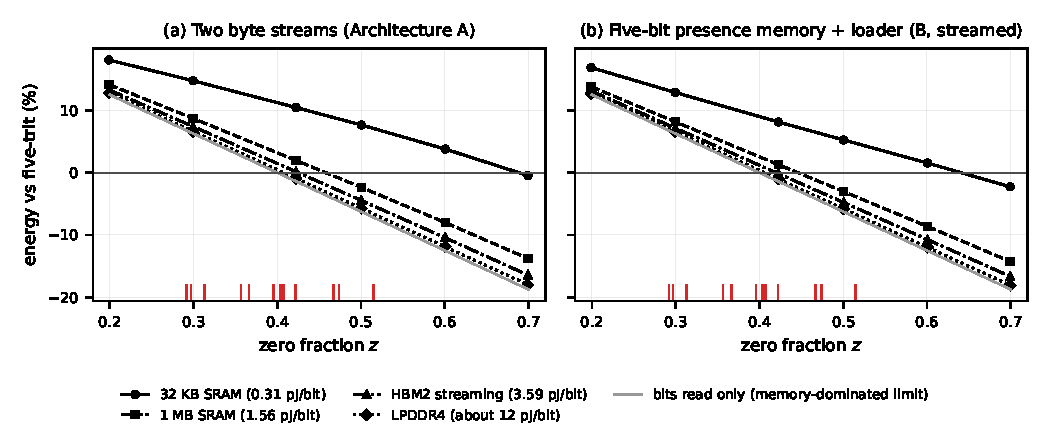
\includegraphics[width=\linewidth]{figures/breakeven.pdf}
\caption{Model: compute plus weight-read energy of the stream-fed
bitmap/sign designs relative to stream-fed five-trit versus zero fraction
(synthetic workloads, smallest netlists meeting 2.0\,ns). Compute energies
are simulated; memory energies per bit are published or literature-derived values. The gray line
is the limit set by bits read alone. Red ticks mark the zero fractions of
the 13 analyzed checkpoints.}
\label{fig:breakeven}
\end{figure}

Table~\ref{tab:system} and Figure~\ref{fig:breakeven} show two regimes among
the tested checkpoints. The nine quantization-aware or fine-tuned models
provide little or no gain: only those above 40\% zeros read fewer bits with
the bitmap format, the largest modeled
saving is 1.3\% of projection-engine plus ternary-symbol weight-read energy (BitNet 2B4T, 0.5\% after adding the output-head weight read), and the five below 37\% zeros lose in every configuration. The
CAT-Q Qwen3 checkpoints lie beyond it: with weights streamed from LPDDR4 at
2.0\,ns, Architectures~A and B-streamed save 3.7--6.7\%, while Architecture~B with
resident weights saves 2.7--5.4\% at the 1\,MB 45\,nm SRAM energy point.
The output-head weight read reduces these savings: CAT-Q keeps the head in 16-bit floating
point, where it accounts for about half the modeled weight bytes read per token for Qwen3-8B. Adding CAT-Q's common 16-bit scale read per 128 ternary weights lowers the A/B-streamed LPDDR4 saving across the tested clocks from 3.7--6.8\% to about 3.4--6.3\%. Adding the output-head weight read as well leaves about
1.9--2.1\% savings, and the best configuration (B resident restricted to
on-chip SRAM) about 2.2\% for all three Qwen3 checkpoints. The worst tested bitmap/sign configuration for every checkpoint costs 17--22\% more
than five-trit.

If five-trit packing restarts at every 128-weight group, as a five-trit
engine for group-scaled weights like CAT-Q's may require, five-trit costs
1.625 bits per weight and the best bitmap/sign case for each checkpoint improves by about
1.3--1.5 percentage points (best case: $-8.5\%$ for
Qwen3-1.7B, $-2.9\%$ for BitNet 2B4T). At the model's illustrative 34.1\,GB/s modeled weight-bandwidth point, five-trit's weight-bandwidth-bound rate is about 13--102 tokens per second across the 13 checkpoints. At a 2.0\,ns clock, matching those rates requires about 0.025--0.069\,mm$^2$ of replicated five-trit engine standard cells in this pre-layout model, excluding memories. Above that compute provision, this weight-only throughput model is bandwidth-bound and follows the modeled weight bytes read, changing by about $-3.2\%$ to $+2.3\%$ across the tested checkpoints.

\section{Discussion}

When only the compute engines are compared, the direct bitmap/sign datapath can shorten the critical path, but the presence mask does not systematically reduce energy per weight. The five-trit decoder already suppresses zero weights before the same adder tree, so arbitrary element-level zeros remove no additional arithmetic in this five-lane GEMV design. Feeding separate presence and variable-rate sign streams then adds area and energy. Natural sparsity therefore changes the weight representation more than the arithmetic performed by the core.

The system-level value is governed mainly by compression. Against continuous five-trit packing, the bitmap/sign stream becomes smaller above 40\% zeros and larger below it. This explains the two regimes in the measured checkpoints: models near the threshold have little or no benefit, while higher-zero CAT-Q Qwen3 models benefit more when weights are read from expensive off-chip memory. Architecture~B shows that the feeding organization can reduce some overhead when compressed weights are already resident on chip, but that case does not include the capacity or area needed to store a multi-billion-weight model. Hardware intended to cover both low- and high-zero regimes may therefore benefit from supporting both formats.

The bitmap/sign storage format comes from BITCOS \cite{georganas2026bitcos}; its 37.5\% storage break-even applies when five-trit packing restarts every 128 weights, while the 40\% threshold used in the main experiments follows from the continuous 1.6-bit baseline. Zero-gated arithmetic and five-trit hardware decoding are also established. This study contributes the matched RTL and gate-level comparison, including feeding hardware, together with the observation that the mask provides no consistent compute-energy saving and the break-even analysis using exact statistics from real checkpoints.

\section{Limitations}

All hardware numbers are pre-layout: synthesis and static timing in the
open Nangate45 library at the typical corner, and power from zero-delay
gate-level simulation without glitches, wires, clock tree or clock gating.
A modern node, layout, or a different library could shift the percentages;
the structural fact that the five-trit zero code already gates the adder
tree does not depend on them. Each comparison is between single engines of
five weights per cycle with 8-bit activations; multi-engine tiles, wider
datapaths and other activation precisions are outside this matched study. Compute energies
come from synthetic activations and independent random zeros; on the 24
sampled BitNet rows the interpolated synthetic ratio agrees with the one
simulated on the real rows within 0.7 percentage points. Memory-energy points are published estimates and model-derived values, plus a separately computed CACTI sensitivity point. The LPDDR4 point comes from DramDSE modeling, and the HBM2 points from a floorplan-based energy model \cite{ha2018dram,oconnor2017fgdram}. The CACTI sensitivity value is checked in, but the original CACTI input configuration was not archived.
The memory model is linear in payload bits: it assumes the cited per-bit energy applies proportionally to the modeled stream and does not simulate access granularity, burst utilization, background-energy scaling, or actual memory-port transactions. A five-bit-wide memory is assumed to cost the same per bit as a byte-wide
one, and memory macros are not synthesized. The B-resident model-wide projection
scenario uses per-bit SRAM energy to test sensitivity and does not model the
on-chip capacity or area required to hold an entire multi-billion-weight
model. The stream-size calculations omit redundant prefetch reads at row boundaries and final byte or loader-block rounding. Tail positions use the tensor-average compute estimate rather than separately simulated padding activity. The main pointer-free model assumes sequential row consumption with a carried sign cursor; the current RTL instead receives each row's start address from outside the synthesized block. If arbitrary row access is required, row-start sign pointers or equivalent metadata/control must be supplied. Row-start sign pointers are therefore excluded from the model-wide projection model;
for the exact BitNet storage calculation, one 32-bit pointer per row plus one terminal pointer per tensor reduces
the block-128 storage advantage from 2.90\% to 2.25\%. The model-wide projection
estimate assumes batch size one with every modeled weight read once per token;
larger batches reuse weights and favor five-trit. The power traces and model-wide projection model also use a matched one-cycle prefill for every fed engine. The bitmap feeders require this cycle, while the five-trit feeder does not; removing it would reduce five-trit execution cycles by about 0.10--0.28\% across the 13 checkpoints and would slightly favor five-trit. CAT-Q's per-128-weight scales are not modeled in the synthesized datapaths. A scale-aware implementation would need either to preserve 128-weight scale-group boundaries (128 is not divisible by five) or to handle a five-lane cycle that crosses a scale boundary. That logic, the scale arithmetic, and its energy are outside this study; the CAT-Q percentages should therefore be read as ternary-symbol-path estimates. Adding the common scale reads alone gives the sensitivity reported above.
The synthesized feeders use 16-bit local memory addresses (64 KiB byte-address space), so the hardware results represent tiled/local buffers rather than direct full-model addressing. Wider counters and tile-control logic are not modeled; this can matter because Architecture~A has two stream counters while five-trit has one. Throughput figures are model upper bounds, not measured tokens per second.
Zero statistics cover the projection weights of 13 checkpoints exhaustively and 18 additional models
by sampling; the screening data also contain seven intermediate TriLM 99M
training checkpoints. For \texttt{bitnet\_b1\_58-large}, the ternary codes are reconstructed from its full-precision latent weights with the stated BitNet absmean rule rather than read from stored ternary codes. Applying that rule to two layers of the packed BitNet 2B4T reference disagrees on 0.72\% of weights, all within $\pm1/256$ of the rounding threshold and with no sign disagreements, so the reported zero fraction for this checkpoint should be understood as quantizer-derived. Two first-layer TriLM tensors have zero fractions near
97\%, outside the 20--70\% synthetic power sweep, so their model-wide projection
compute energies use linear extrapolation from the high-sparsity end of the sweep. The checkpoint survey is not exhaustive.

\section{Conclusion}

Natural zeros in pretrained ternary LLMs can be exploited directly with a fused presence-bitmap and compact-sign GEMV engine, but the matched hardware shows that the presence mask does not itself reduce compute energy because five-trit decoding already suppresses zero-weight contributions before the same adder tree. Against continuous five-trit packing, bitmap/sign storage becomes smaller above 40\% zeros, so its consistent advantage is reduced weight traffic rather than reduced arithmetic; the quantization-aware or fine-tuned checkpoints tested here gain little or nothing, while the higher-zero CAT-Q Qwen3 checkpoints can retain a small benefit under expensive off-chip streaming. Under the assumptions tested here, natural ternary sparsity is therefore a niche optimization rather than a general reason to replace five-trit packing.

\section*{Reproducibility}

All RTL, testbenches, reference models, synthesis, timing and power scripts,
checkpoint analysis scripts, raw results and the figure-generation script are
in the public repository
\url{https://github.com/jacobzymet/natural-sparsity-ternary-llms}. The EDA flow is packaged in a
Docker image (Yosys~0.33, OpenSTA~3.1.0, Icarus Verilog~12, Nangate45). The repository records the scripts, commands, tool versions, checkpoint
revisions, file hashes, and checked-in data used to trace the reported results. Reproduction commands and the data layout are in
\path{REPRODUCING.md}.

\bibliographystyle{plain}
\bibliography{references}
\end{document}
